\documentclass[10pt]{article}
\usepackage{graphicx}
\usepackage{epstopdf}
\DeclareGraphicsRule{.tif}{png}{.png}{`convert #1 `basename #1 .tif`.png}
\usepackage{enumerate}
\usepackage{fullpage}
\usepackage{float}
\restylefloat{table}
\restylefloat{figure}

\begin{document}
\pagenumbering{gobble}

\begin{figure}[H]
	\begin{center}
	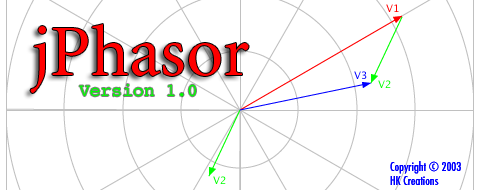
\includegraphics{../../images/jPhasorLogo}
	\end{center}
\end{figure}

\section*{Readme Sections}
\begin{itemize}
	\item What is jPhasor?
	\item Where do I get it?
	\item How do I run it?
	\item How do I use it?
	\item Known Bugs
	\item Planned Features
	\item Licensing Information
	\item Bug Reports
\end{itemize}

\section*{What is jPhasor?}
jPhasor is a program in Java to draw phasors of voltage and current onto a polar graph. 
If you don't know, a phasor is basically just a vector, but instead of x-y components it is 
made up of real and imaginary parts. In polar coordinates these are transformed to magnitude and phase.
\\ \\
Also, as a side bonus, jPhasor can also use this polar plot to draw power triangle diagrams. 
A power triangle consists of the real power, the imaginary power, and the apparent power. 
These are also drawn as vectors on the real-imaginary plane.

\section*{Where do I get it?}
The best place to find jPhasor is at http://www.hkcreations.org/ under the Projects section.
Eventually this program may get a home at Sourceforge.net, but for now this is where to find
jPhasor.

\section*{How do I run it?}
jPhasor is distributed with both a precompiled jar file, as well as with the source in case you wish to compile it yourself. It is very important that you have a Java Runtime Environment (JRE) or Java Software Development Kit (SDK) installed on your machine before you attempt to run jPhasor, as jPhasor will not run without one of these. Windows, Linux, and other *nix users can get the newest JRE or SDK at http://java.sun.com/downloads/ though you may wish to choose something other than 1.4.1, as there is a serious bug with that version (see Known Bugs below).
\\ \\
For Windows and Mac OS X systems, you should just be able to double-click on the jPhasor.jar file to run it. This may also work on Linux, but I do not know. If you cannot double-click the file, you can still run it from the command line, using this statement: {\tt java -jar jPhasor.jar} while you are in the jPhasor directory.

\section*{How do I use it?}
Once jPhasor is running, the interface should be fairly self explanatory. To add a phasor, click the Add... button under either the voltage or current list on the right side of the window. This brings up a dialog where you can fill in values for Name, Magnitude, Phase, and Color of your phasor. Then click OK, and the phasor appears on the graph.  Once the phasor is in the list, you may select it and activate/deactivate, edit, or remove the selected phasor.
\\ \\
The 4 text fields in the bottom right corner control the scaling of the graph, as well as the
display of the axes. Voltage and Current scaling may be changed independently of one another. Currently none of the drop-down menus of units have any function (see Planned Features for more info).

\section*{Known bugs}
Right now jPhasor seems to be stable, but a program is never really free of bugs. Here are the ones that are currently known to the development staff:
\begin{itemize}
	\item There is an issue with jPhasor and Java v1.4.1 where the Add Phasor Dialog box is not laid out properly. We are currently investigating this bug to try and find a solution. As a workaround, jPhasor seems to work properly under any other Java2 version (1.2 - 1.4.0). This issue will be rectified as soon as possible.
\end{itemize}

\section*{Planned Features}
\begin{itemize}
	\item Allowing users to add phasors together using the Add To menu in the phasor dialog box.
	\item Allowing users to select units for individual phasor magnitudes, as well as for the scaling, to properly display magnitudes with units.
	\item Allowing users to enter phase angles in radians as well as degrees.
\end{itemize}

\section*{Licensing Information}
\begin{quotation}
{\tt
\noindent This program is free software; you can redistribute it and/or modify it under the terms of the GNU General Public License as published by the Free Software Foundation; either version 2 of the License, or (at your option) any later version.\\

\noindent This program is distributed in the hope that it will be useful, but WITHOUT ANY WARRANTY; without even the implied warranty of MERCHANTABILITY or FITNESS FOR A PARTICULAR PURPOSE.  See the GNU General Public License for more details. \\

\noindent You should have received a copy of the GNU General Public License along with this program; if not, write to the Free Software Foundation, Inc., 59 Temple Place, Suite 330, Boston, MA  02111-1307  USA
}
\end{quotation}
The Full GPL text can be found in the file LICENSE which should have accompanied this ReadMe.

\section*{Bug Reports}
Please send bug reports to bugs@hkcreations.org. Include the program and as detailed a description as  you can provide. Other contact information may be found at the HK Creations website at http://www.hkcreations.org/
\end{document}